\documentclass{standalone}
\usepackage{amsmath}
\usepackage[dvipsnames]{xcolor}
\usepackage{tikz} 
\usetikzlibrary{arrows, decorations.markings,decorations.pathreplacing,angles,quotes}
\usepackage{microtype}
\usepackage{fourier}

%include other needed packages here   
\begin{document}

\begin{tikzpicture}
% include your tikz code here
    		\node[anchor=south west,inner sep=0] (Bild) at (0,0) {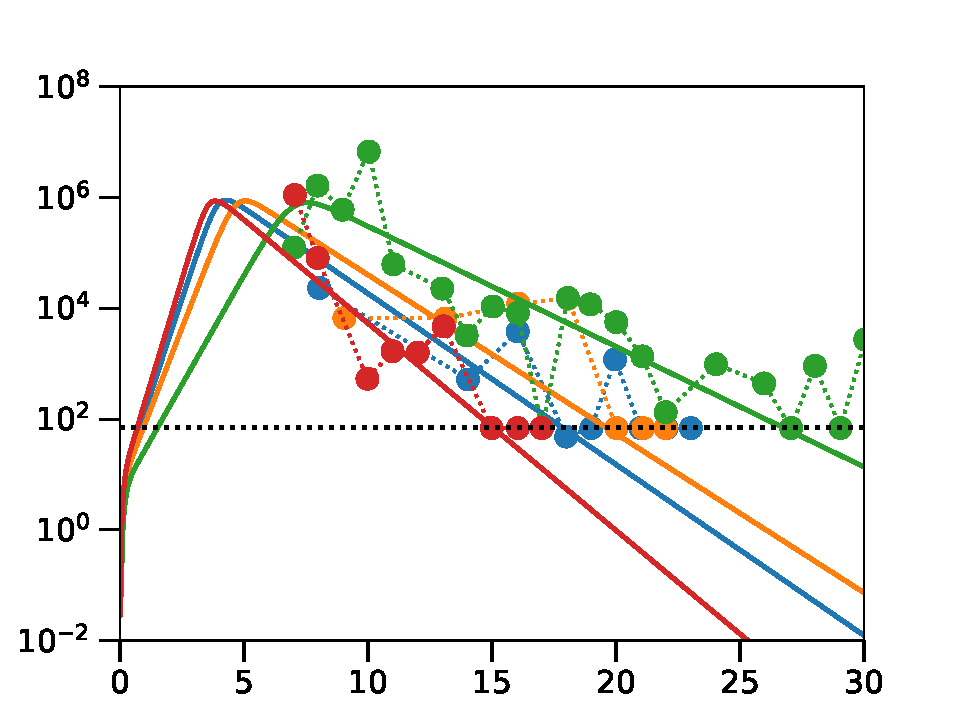
\includegraphics[scale=0.39]{fig1_blank.pdf}};
   		\begin{scope}[x=(Bild.south east),y=(Bild.north west)]
        	\draw (0.55,-0.035) node {time after infection (days)};
        	\draw (-0.01,0.5) node [rotate=90] {virus (copies.mL$^{-1}$)};
        	%\draw[blue,thick] (0.175,1.05) -- node[right=6pt] {\scriptsize \color{black} reducing burst size $B$} (0.225,1.05);
        	%\draw[orange,thick] (0.175,0.98) -- node[right=6pt] {\scriptsize \color{black} reducing infectivity $\beta$} (0.225,0.98);
        	%\draw[black,thick] (0.725,1.085) -- node[right=6pt] {\scriptsize \color{black} $V_0=1$} (0.775,1.085);
        	%\draw[black,thick,dashed] (0.725,1.015) -- node[right=6pt] {\scriptsize \color{black} $V_0 = 10$} (0.775,1.015);
        	%\draw[black,thick,dotted] (0.725,0.945) -- node[right=6pt] {\scriptsize \color{black} $V_0 = 100$} (0.775,0.945);
    		\end{scope}
\end{tikzpicture}

\end{document}